\section{Ковёр Серпинского}

\subsection{Определение}

Ковёр Серпинского — это фрактальная фигура на плоскости, которая строится путём последовательного удаления частей из исходного квадрата. 

\subsection{Метод построения}

\begin{enumerate}
    \item Начинаем с квадрата единичного размера.  
    \item Делим его на $3\times3$ равных частей.  
    \item Удаляем центральный квадрат.  
    \item Повторяем процесс для всех оставшихся квадратов.  
    \item Продолжаем до достижения заданного уровня итерации $n$.  
\end{enumerate}

\subsection{Визуализации}

\begin{figure}[h]
    \centering
    \begin{subfigure}{0.30\textwidth}
        \centering
        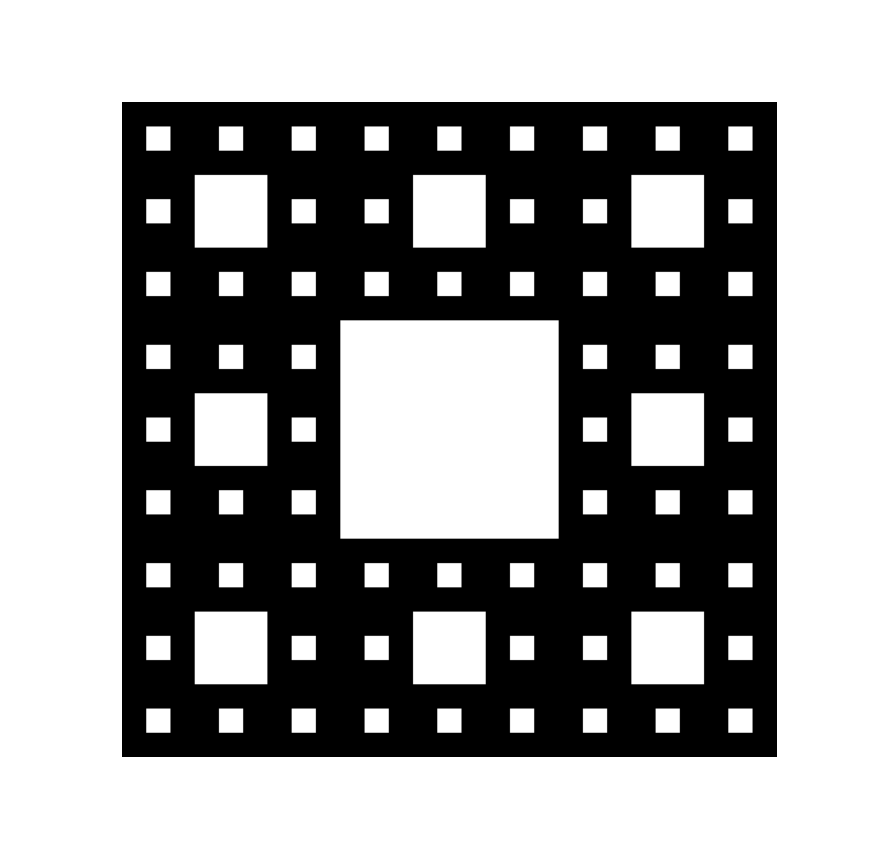
\includegraphics[width=\linewidth]{pic/07.png}
        \caption{Количество итераций - 3}
        \label{fig:julia_detail1}
    \end{subfigure}
    \hfill
    \begin{subfigure}{0.30\textwidth}
        \centering
        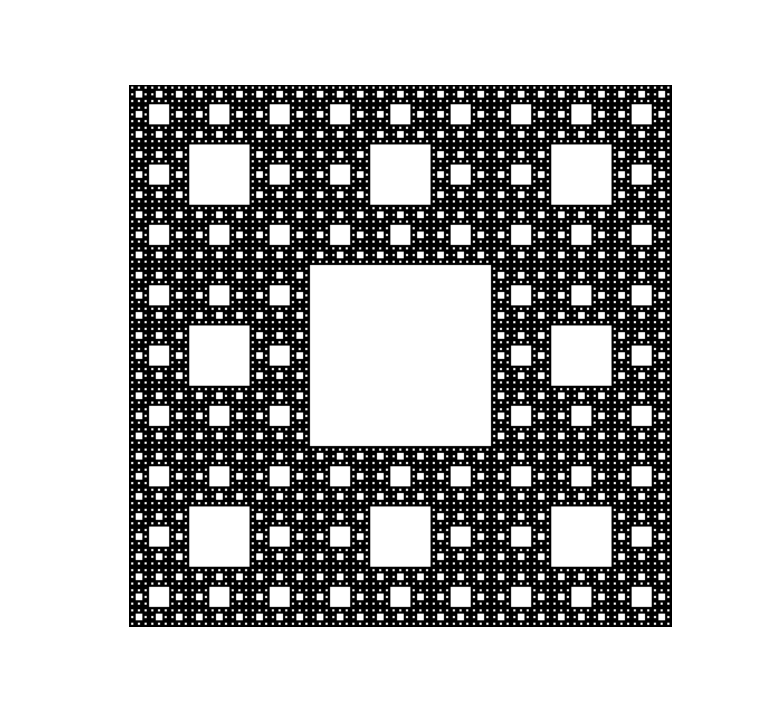
\includegraphics[width=\linewidth]{pic/08.png}
        \caption{Количество итераций - 5}
        \label{fig:julia_detail2}
    \end{subfigure}
    \hfill
    \begin{subfigure}{0.30\textwidth}
        \centering
        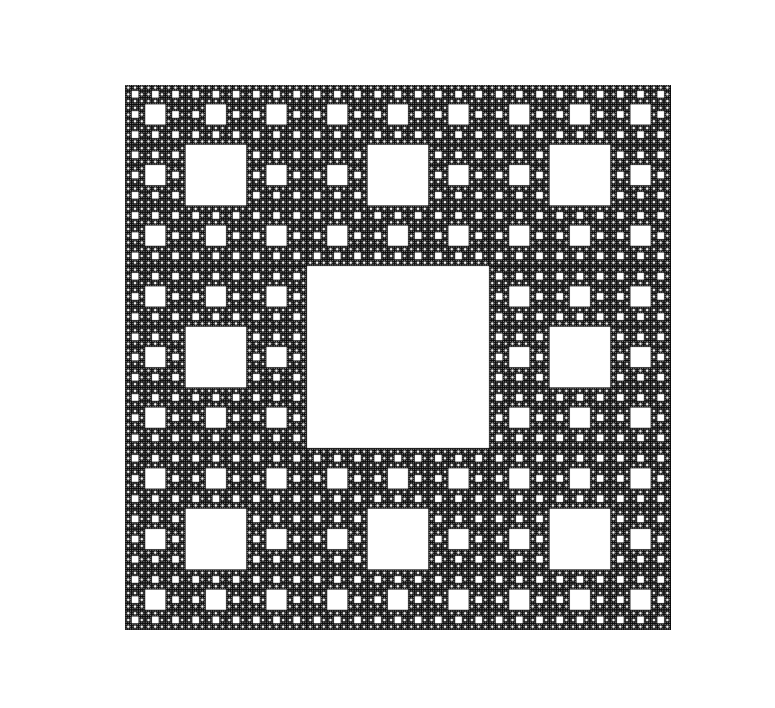
\includegraphics[width=\linewidth]{pic/09.png}
        \caption{Количество итераций - 7}
        \label{fig:julia_detail3}
    \end{subfigure}
    \caption{Визуализации Ковёра Серпинского при разном количестве итераций}
    \label{fig:julia_details}
\end{figure}